\documentclass[12pt,xcolor=dvipsnames]{beamer}
\usetheme{AnnArbor}
\usecolortheme{crane}

\usepackage{hyperref}   
\usepackage{url}
\hypersetup{urlcolor=red}

\renewcommand{\bibname}{References}
\setbeamertemplate{bibliography item}{[\theenumiv]}

\usepackage{kbordermatrix}
\usepackage{multicol}
\usepackage{verbatim} 
\usepackage{graphics}
\usepackage{graphicx}
\usepackage{tikz}


%Basic Information
\title{Graph Based Storage for Relational Databases}
\author{Adarsh, Ajith, Ashish, Sourabh}
\date{\today}

%--------------------------------------------------------------------------------------
%               TITLE PAGE (Slide 1)
%--------------------------------------------------------------------------------------
\begin{document}
\begin{frame}
\titlepage
\end{frame}
%--------------------------------------------------------------------------------------


%--------------------------------------------------------------------------------------
%               Outline
%--------------------------------------------------------------------------------------
\begin{frame}
\frametitle{Outline}
\begin{multicols}{2}
\tableofcontents[hideallsubsections]
\end{multicols}
\end{frame}

\section{Abstract}
\begin{frame}
\frametitle{Abstract}
\begin{itemize}
  \item To develop a data storage system based on graph structure in order to optimize the query execution time especially join queries and eliminate some sort of data redundancy in a relational model while retaining other advantages of relational database system in terms of performance of other queries.
\end{itemize}
\end{frame}

\section{Overview of Model}
\begin{frame}
 \frametitle{Overview of the Model}
 \begin{itemize}
  \item<1-> A database consist of multiple tables
  \item<2-> Each table is a collection of domains
  \item<3-> Each table contains list of main node records
 \end{itemize}
\end{frame}

\begin{frame}
\begin{figure}[t]
 \centering
 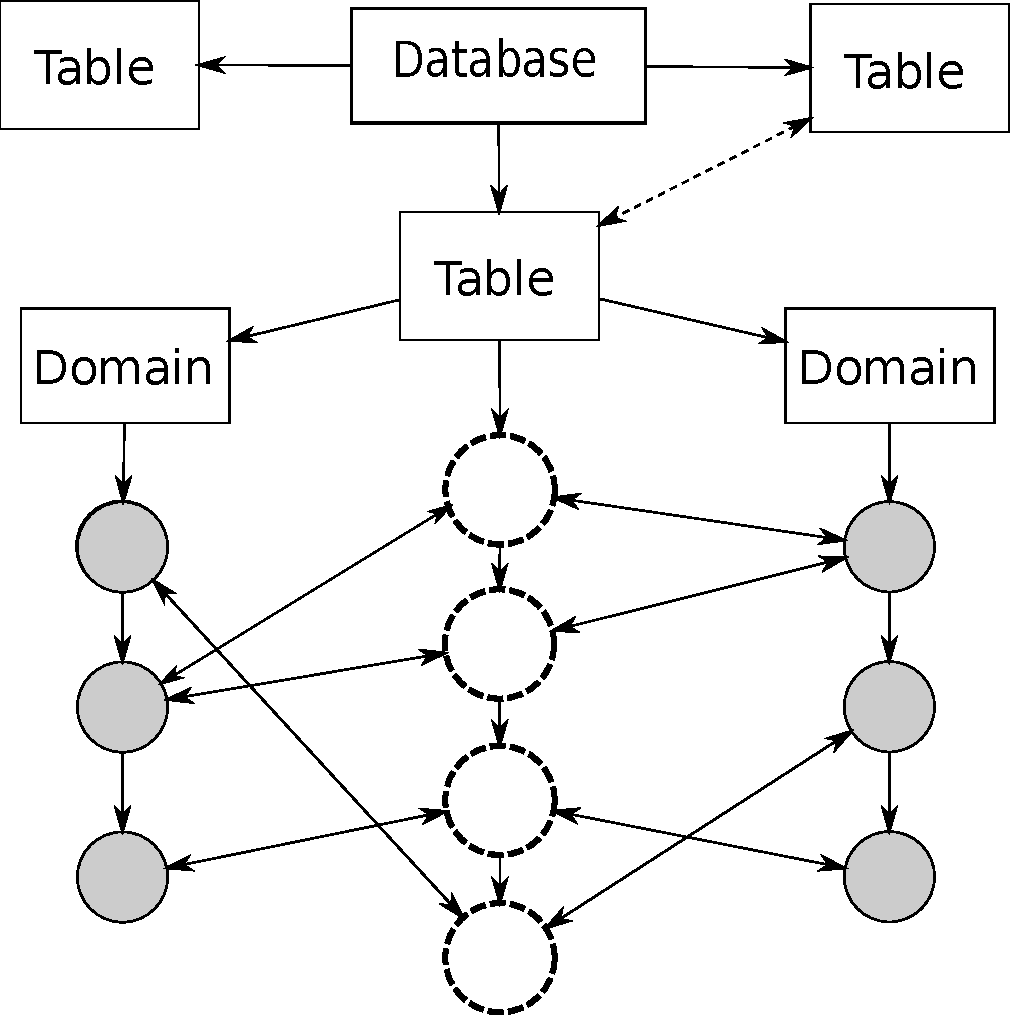
\includegraphics[width=0.7\textwidth]{pics/model.pdf}
 \caption{Overview of Proposed Graph Based Storage}
 \label{fig:overview}
\end{figure}
\end{frame}

\begin{frame}
 \frametitle{Overview of the Model}
 \begin{itemize}
  \item<1-> A database consist of multiple tables
  \item<1-> Each table is a collection of domains
  \item<1-> Each table contains list of main node records
  \item<2-> Each Domain is collection of attribute nodes
  \item<3-> Each attribute node contains the actual data elements
 \end{itemize}
\end{frame}

\section{Primary Key}
\begin{frame}
 \frametitle{Primary Key}
 \begin{figure}
 \centering
 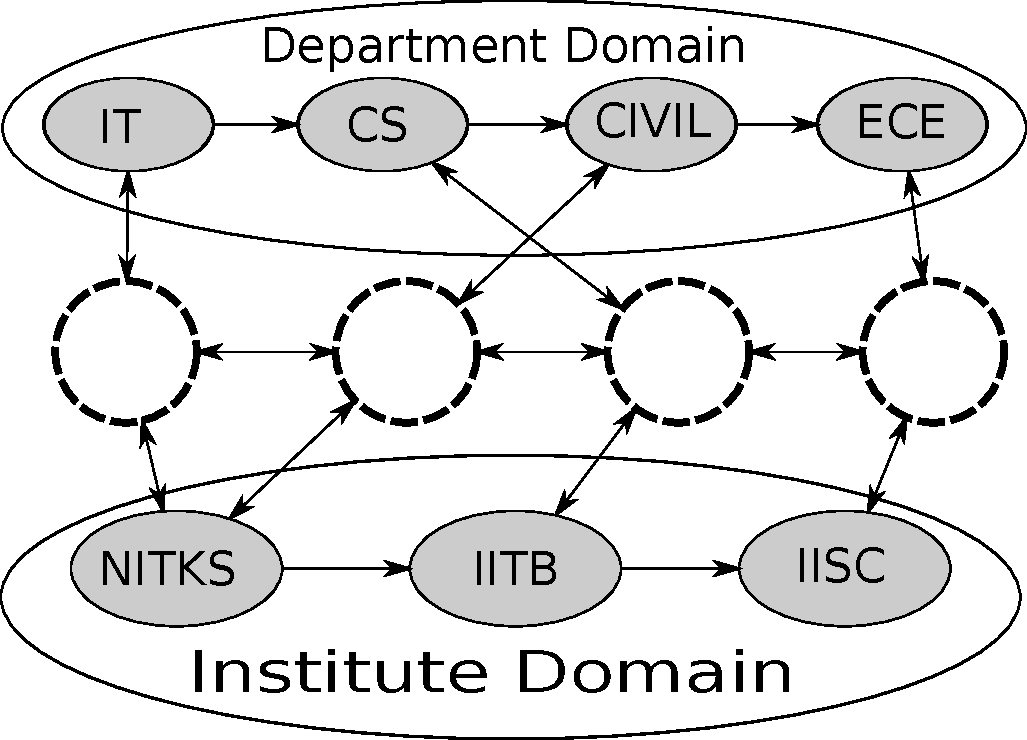
\includegraphics[width=0.7\textwidth]{pics/primary_key.pdf}
 \caption{Primary Keys in Proposed Model}
 \label{fig:primary_key}
\end{figure}
\end{frame}

\section{Foreign Key}
\begin{frame}
 \frametitle{Foreign Key}
 \begin{figure}[h]
 \centering
 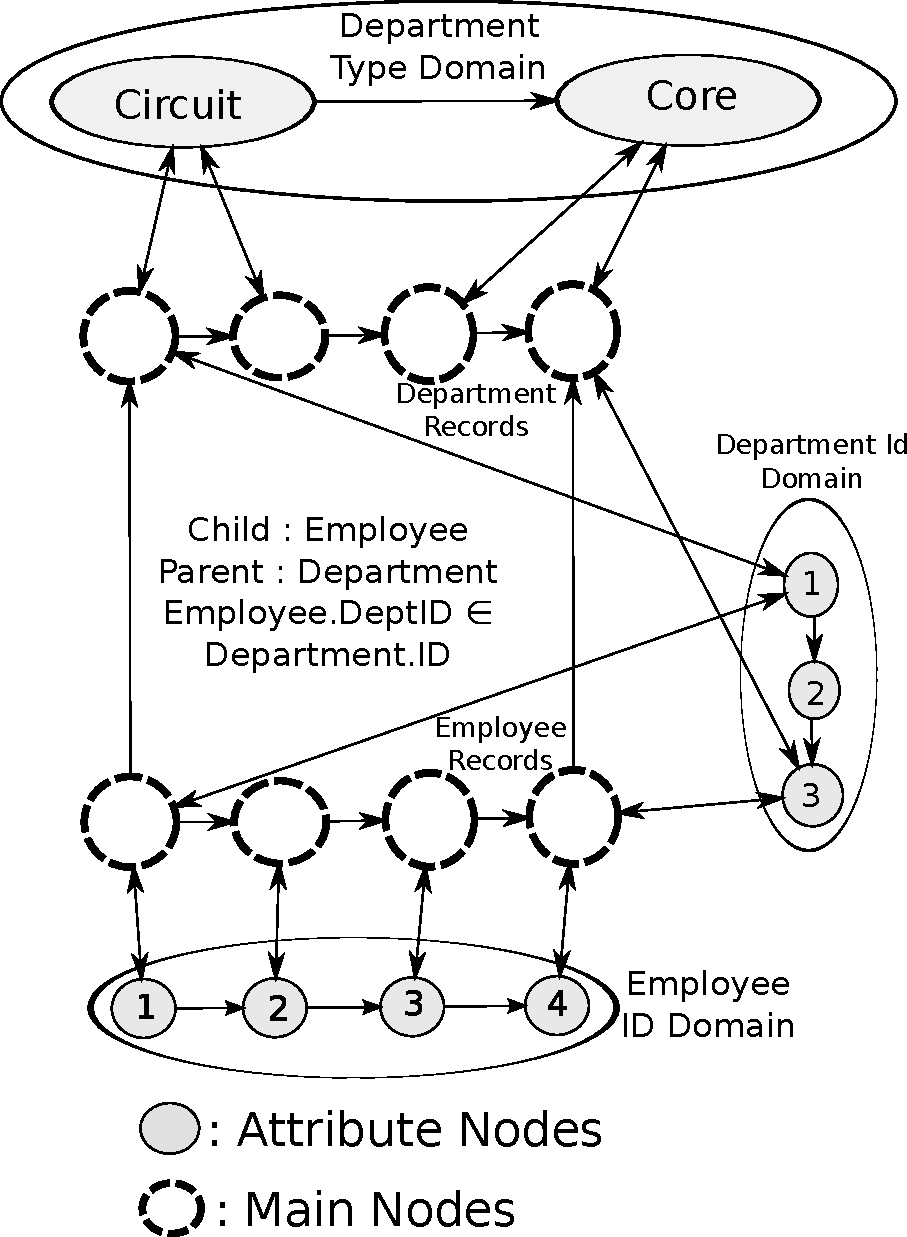
\includegraphics[width=0.45\textwidth]{pics/foreign_key.pdf}
\end{figure}
\end{frame}

\section{Indexing}
\begin{frame}
 \frametitle{Indexing Using Trie}
 \begin{figure}
 \centering
 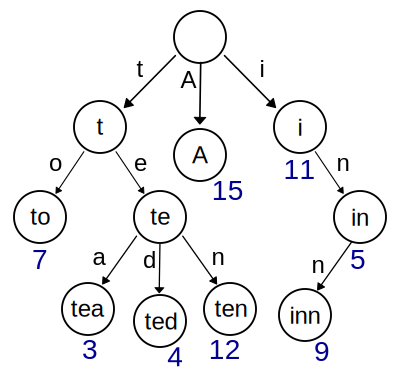
\includegraphics[width=0.5\textwidth]{pics/trie.pdf}
 \caption{Trie Data Structure for Indexing}
\end{figure}
\end{frame}
\end{document}